\documentclass{article}
\usepackage{tikz}
\usetikzlibrary{shapes,arrows,positioning,fit,backgrounds}

\begin{document}

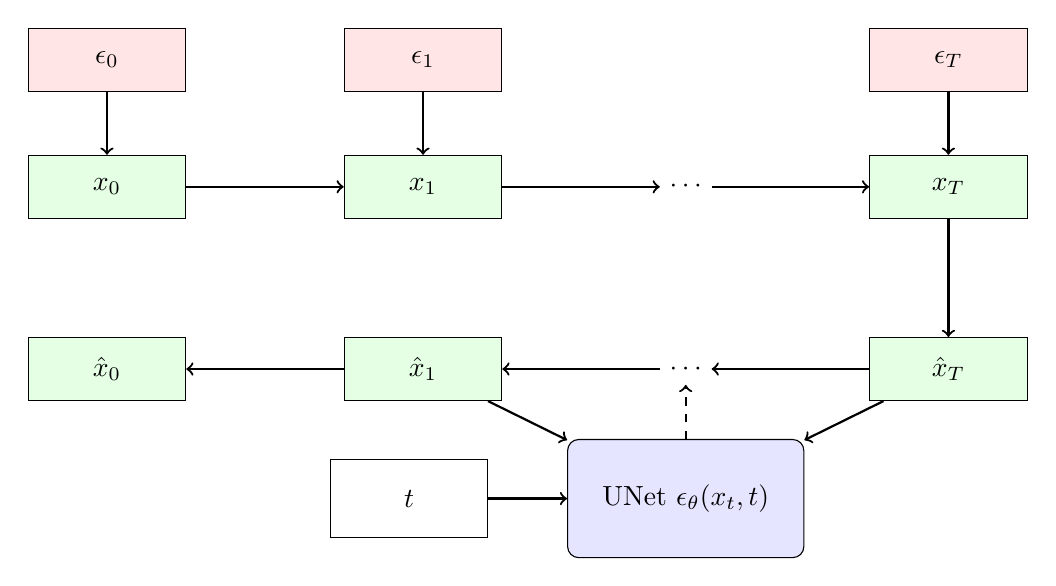
\begin{tikzpicture}[
    node distance=2cm,
    box/.style={rectangle, draw, minimum width=2cm, minimum height=1cm},
    arrow/.style={->, thick},
    unet/.style={rectangle, draw, rounded corners, minimum width=3cm, minimum height=1.5cm, fill=blue!10},
    data/.style={rectangle, draw, minimum width=2cm, minimum height=0.8cm, fill=green!10},
    noise/.style={rectangle, draw, minimum width=2cm, minimum height=0.8cm, fill=red!10}
]

% Forward process
\node[data] (x0) {$x_0$};
\node[data, right=2cm of x0] (x1) {$x_1$};
\node[right=2cm of x1] (dots1) {$\cdots$};
\node[data, right=2cm of dots1] (xt) {$x_T$};

% Noise arrows forward
\node[noise, above=0.8cm of x0] (e0) {$\epsilon_0$};
\node[noise, above=0.8cm of x1] (e1) {$\epsilon_1$};
\node[noise, above=0.8cm of xt] (et) {$\epsilon_T$};

% Forward process arrows
\draw[arrow] (x0) -- (x1);
\draw[arrow] (x1) -- (dots1);
\draw[arrow] (dots1) -- (xt);

% Noise addition arrows
\draw[arrow] (e0) -- (x0);
\draw[arrow] (e1) -- (x1);
\draw[arrow] (et) -- (xt);

% Single UNet
\node[unet, below=3cm of dots1] (unet) {UNet $\epsilon_\theta(x_t, t)$};

% Reverse process
\node[data, below=1.5cm of xt] (rt) {$\hat{x}_T$};
\node[left=2cm of rt] (dots2) {$\cdots$};
\node[data, left=2cm of dots2] (r1) {$\hat{x}_1$};
\node[data, left=2cm of r1] (r0) {$\hat{x}_0$};

% Reverse process arrows
\draw[arrow] (xt) -- (rt);
\draw[arrow] (rt) -- (dots2);
\draw[arrow] (dots2) -- (r1);
\draw[arrow] (r1) -- (r0);

% UNet connections
\draw[arrow] (rt) -- (unet);
\draw[arrow] (r1) -- (unet);
\draw[arrow, dashed] (unet) -- (dots2);

% Time embedding
\node[box, left=1cm of unet] (time) {$t$};
\draw[arrow] (time) -- (unet);

\end{tikzpicture}

\end{document}